%%%%%%%%%%%%%%%%%%%%%%%%%%%%%%%%%%%%%%%%%%%%%%%%%%%%%%%%%%%%%%%%%%%%%%%%
%                                                                      %
%     File: Thesis_Results.tex                                         %
%     Tex Master: Thesis.tex                                           %
%                                                                      %
%     Author: Andre C. Marta                                           %
%     Last modified :  2 Jul 2015                                      %
%                                                                      %
%%%%%%%%%%%%%%%%%%%%%%%%%%%%%%%%%%%%%%%%%%%%%%%%%%%%%%%%%%%%%%%%%%%%%%%%

\chapter{Identifying File-Test Links with Neural Network Embeddings}
\label{chapter:paper2}


\section{Background}

% Explains what embeddings are.
% Advantages in relation to other encoding
%techniques
% Why they are useful
\subsection{Embeddings}
The idea of embeddings is to map high-dimensional categorical variables into a low-dimensional learned representation that places similar entities closer together in the embedding space. This can be achieved by training a neural network. 
\par More commonly, \textit{One-Hot Encoding} - the process of mapping discrete variables to a vector of 0's and 1's - is used to transform categorical variables into inputs that ML models can understand . In fact, one-hot encoding is a simple embedding where each category is mapped to a different vector. However, this technique has severe limitations: (1) Dealing with high-cardinality categories originates ungovernable input and output spaces, and (2) Mappings are "blind", as vectors representing similar entities are not grouped by similarity. 
Therefore to reduce drastically the dimensionality of the input space and also have a more meaningful representation of categories, a supervised learning task can be designed to learn embeddings.

\subsection{Neural Network Embeddings}

% Explains how Embeddings are learned
\par Embeddings are trainable n-dimensional vectors of fixed size that represent a category and by default are initialized with random values. In order to push vectors representing similar objects together, the supervised learning task will predict whether, in this case, a modified file and a test case are linked. 
By doing so, during training, the embedding representation will gradually improve with gradient descent, minimizing the loss of the predictions and making more meaningful entity representations as entities that have similar behaviour will be pointing in the same direction \cite{geron_hands_on}. In the case of a neural network embedding, it's parameters - the weights - are the embedding components, that are adjusted by backpropagation \footnote{Algorithm for Supervised Learning of Artificial Neural Networks with Gradient Descent}. 


\section{NNE-TCP Approach}
% Summarize section
% Give main lines of the approach
% Enumerate steps that are taken
%

In this section, our approach is presented with detail, explaining how both test-case and file embeddings can be learned from historical data, based on the assumption: Files that cause similar tests to transition, are similar to each other. First, a brief description of what embeddings are is provided, and then an in-depth walkthrough of the implementation of NNE-TCP.

\subsection{Implementation}
% Approach Steps
% Model Description

The NNE-TCP approach is sustained by a predictive model that tries to learn whether a modified file and a test-case are linked or not. The learner is used to make new predictions on unseen data and create test schedules that prioritize test-cases  more likely to be related with files modified in a given revision. The implementation was done with the Python Deep Learning Library - Keras \cite{chollet2015keras}. The steps taken to develop the framework are summarized below: 
\begin{enumerate}
	\item Load and Clean Dataset.
	\item Create Training Set.
	\item Build Neural Network Embedding Model.
	\item Train Neural Network Model.
	\item Evaluate Model's Performance.
	\item Visualize Embeddings using dimensionality reduction techniques. 
\end{enumerate}

% 1)
The dataset should contain records of the files modified in every revision, as well as test cases that suffered transitions. 
Data cleaning is increasingly important as development environments become more dynamic, fast-paced and complex. Dealing with modified file and test-case records can have noise associated. Since these elements are simply files, they can become outdated, deprecated, duplicated, renamed or unused. Therefore, eliminating redundant as well as files/tests that have not been modified/applied recently, constitutes a solid data cleaning strategy.
\\

% 2)
After loading and cleaning the dataset, in order for the model to learn the supervised learning task, it needs a training set. It will be composed by pairs of the form: $(file, test, label)$. The label will indicate the ground-truth of whether the pair is or is not present in the data. 
\\

To create the training set, we need to iterate through each revision and store all pair-wise combinations of files and test-cases in a list. Nonetheless, because the dataset only contains positive examples of linked pairs, there is the need to generate negative examples, i.e. file-test pairs that are not linked, in order to create a more balanced dataset. For the positive samples - pairs that appear in the data - the label is set to 1, whereas for negative examples - pairs that are not in the data - the label is set to $0$, for classification or $-1$ for regression. We define that a negative example occurs when a certain file is modified, but a test-case status remained unchanged, i.e. did not transitioned. Moreover, to generate a balanced dataset and there are, for example, 10 positive pairs in a revision, other 10 unique pairs of modified files and test-cases not involved in transitions are randomly chosen to form the negative examples.
\\

% Data Generator 
As a result of having to create balanced examples for every revision and specially when dealing with large datasets, it could become unpractical, in terms of memory and processing, to store and generate the whole training set at once. Consequently, to alleviate the issue of having to store large amounts of data and overcome limited computer resources, the Keras Class \textit{Data Generator} offers an alternative to generate data \textit{on-the-fly} - one batch \footnote{subset of the entire dataset} of data at a time. Once the weights are updated for every batch, an epoch \footnote{number of passes through the entire dataset} has passed. 
\\

The Data Generator class has parameters to be adjusted: the batch-size, comprising the number of steps to be taken in an epoch; the shuffle flag, that if true mixes the order of the batches, once a new epoch begins; the negative-ratio, that represents the dataset class balance ratio. If it is equal to $1$, then there are as many positive examples as there are negative, if it is equal to $2$, then there are twice as many negative examples, as there are positives and so on. \
\\

% 3)
Now that a training set is created, the next step is to build the learning model's architecture. The inputs of the neural network are (file, test) pairs, converted to integers and the output will be a prediction of whether or not there is a link. The model is composed by the following layers and depicted below in \ref{keras_model}: 

\begin{itemize}
	\item Input: 2 neurons for each file and test-case in a pair
	\item Embedding: map each file and test-case to a n-dimensional vector.
	\item Dot: calculates the dot product between the two vectors, merging the embedding layers.
	\item Reshape: Layer to reshape the dot product into a single number.
	\item $\lbrack Optional\rbrack$ Dense: generates output for classification with sigmoid activation function \footnote{ Commonly known as logistic function $S(x) = \frac{1}{e^{-x} +1}$}.
\end{itemize}

\begin{figure}[h]
	\centering
	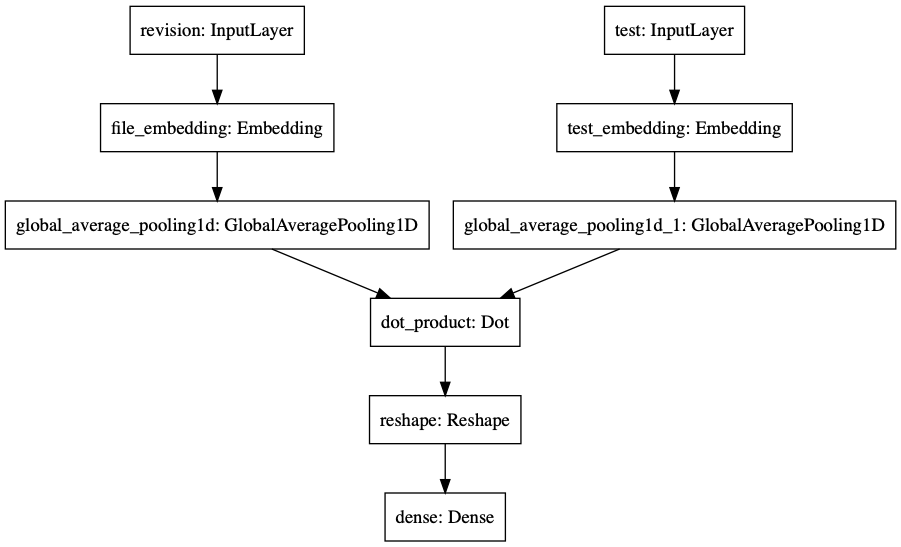
\includegraphics[width=8cm]{figures/model.png}
	\caption{Neural Network Embedding Model Architecture}
	\label{keras_model}
\end{figure}

After converting each file and test-case to a unique integer, they are fed as inputs to the neural network. Afterwards, the embedding layer deals with representing each one of them as a vector in n-dimensional space. Then, the two representations need to be combined into a single number, by calculating the dot product - pair-wise multiplication and sum over all elements. This number will be the output, for a regression task, which will then be compared with the true label ($-1$ or $1$). Then, by calculating the loss function - the mean squared error - the distance between the true and predicted labels will be minimized, by readjusting the model's weights.
\\
For classification, because the label is either $0$ or $1$, a Dense layer with a sigmoid activation function needs to be added to the model  to squeeze the output between $0$ and $1$. The chosen loss function was the binary cross-entropy, that measures the similarity between binary classes \cite{chollet2015keras}. 
% For loss functions I could go more in depth and write the formulas for each one and discuss limit cases. Here information is ommited but will be in depth in thesis.
\\

Once the model is built, the next step is to train it with examples produced by the Data Generator, for a certain number of epochs. At this stage, weights are updated such that the according loss function (depending on choosing classification or regression) is minimized and the accuracy of predicting if the pair is positive or negative is maximized. If the algorithm converges, the model is ready to make predictions on unseen data and produce meaningful representations of files and test-cases embeddings.
\\

% 5)
The metrics used to evaluate the model's performance, are the accuracy and the APFD. Focusing on the latter, the ultimate goal is to maximize APFD in order to apply relevant tests as soon as possible. 
Since there is no information \textit{apriori} of which test-cases will pass or fail in a given revision, the testing set will only be composed by combinations the files that were modified and all test-cases. Then the algorithm will rank test-cases by likelihood of being linked to each modified file, resulting in a matrix of scores $n \times m$ where $n$ corresponds to the number of files that were modified in the current revision and $m$ the total number of test-cases.  
Subsequently, to create a test ordering the maximum value is chosen for each column, resulting in a single vector of size $m$ and test-cases are ranked by descending order, from higher score to lower. Finally, the APFD metric is calculated by applying test-cases according with the obtained test schedule and evaluating when faults were discovered.
\\

% 6)
Lastly, another useful application of training embeddings is the possibility of plotting them in a reduced dimensional space for intuition about entity representation. 
\\

Since embeddings are represented in a n-dimensional manifold, one has to resort to manifold reduction techniques to represent elements in 2D or 3D. This can be done by using T-SNE: t-Stochastic Distributed Neighbors Embedding \cite{tsne} or UMAP: Uniform Manifold Approximation and Projection \cite{umap}, which are both utilized to map vectors to lower dimensional spaces, while preserving the structure of the manifold and the relative distances between elements.


\section{Experimental Setup}

An experimental evaluation of our approach to the algorithm is presented, with a brief description of the dataset used, the corresponding cleaning steps applied and the results obtained: both prioritizations and embedding representation in 2D space.

\subsection{Data Description} 

The dataset used to trained NNE-TCP consists on historical data collected from the SVN log \footnote{Document that displays commit log messages.} for a team of around 90 developers, belonging to a large company of the financial sector. The data was collected over a period of four years and contains information relative to the commits, tests and modified files. In short, the dataset contain over 4000 commits, 10800 files and 4000 test-cases.
Each dataset row has 3 columns: the first with the commit identifier, which is a number, then a list of the files modified in that commit and lastly, a list of the tests that transitioned.
It is worth noting that for privacy purposes the data was anonymized and therefore the dataset does not contain any information that corresponds to reality. 

\subsection{Data Cleaning}

Data Cleaning has 3 steps: the date from which we consider relevant files, the individual frequency of each element - files that appear few times are likely to be irrelevant or noisy - and, finally, the frequency of the pair itself - rare pairs may have occurred by chance. To remove the noise from the data we want the average number of occurrences per file to be larger - we want more density of relevant files and tests. The density varies according to the surface plot depicted in \ref{surf}:

\begin{figure}[h]
	\centering
	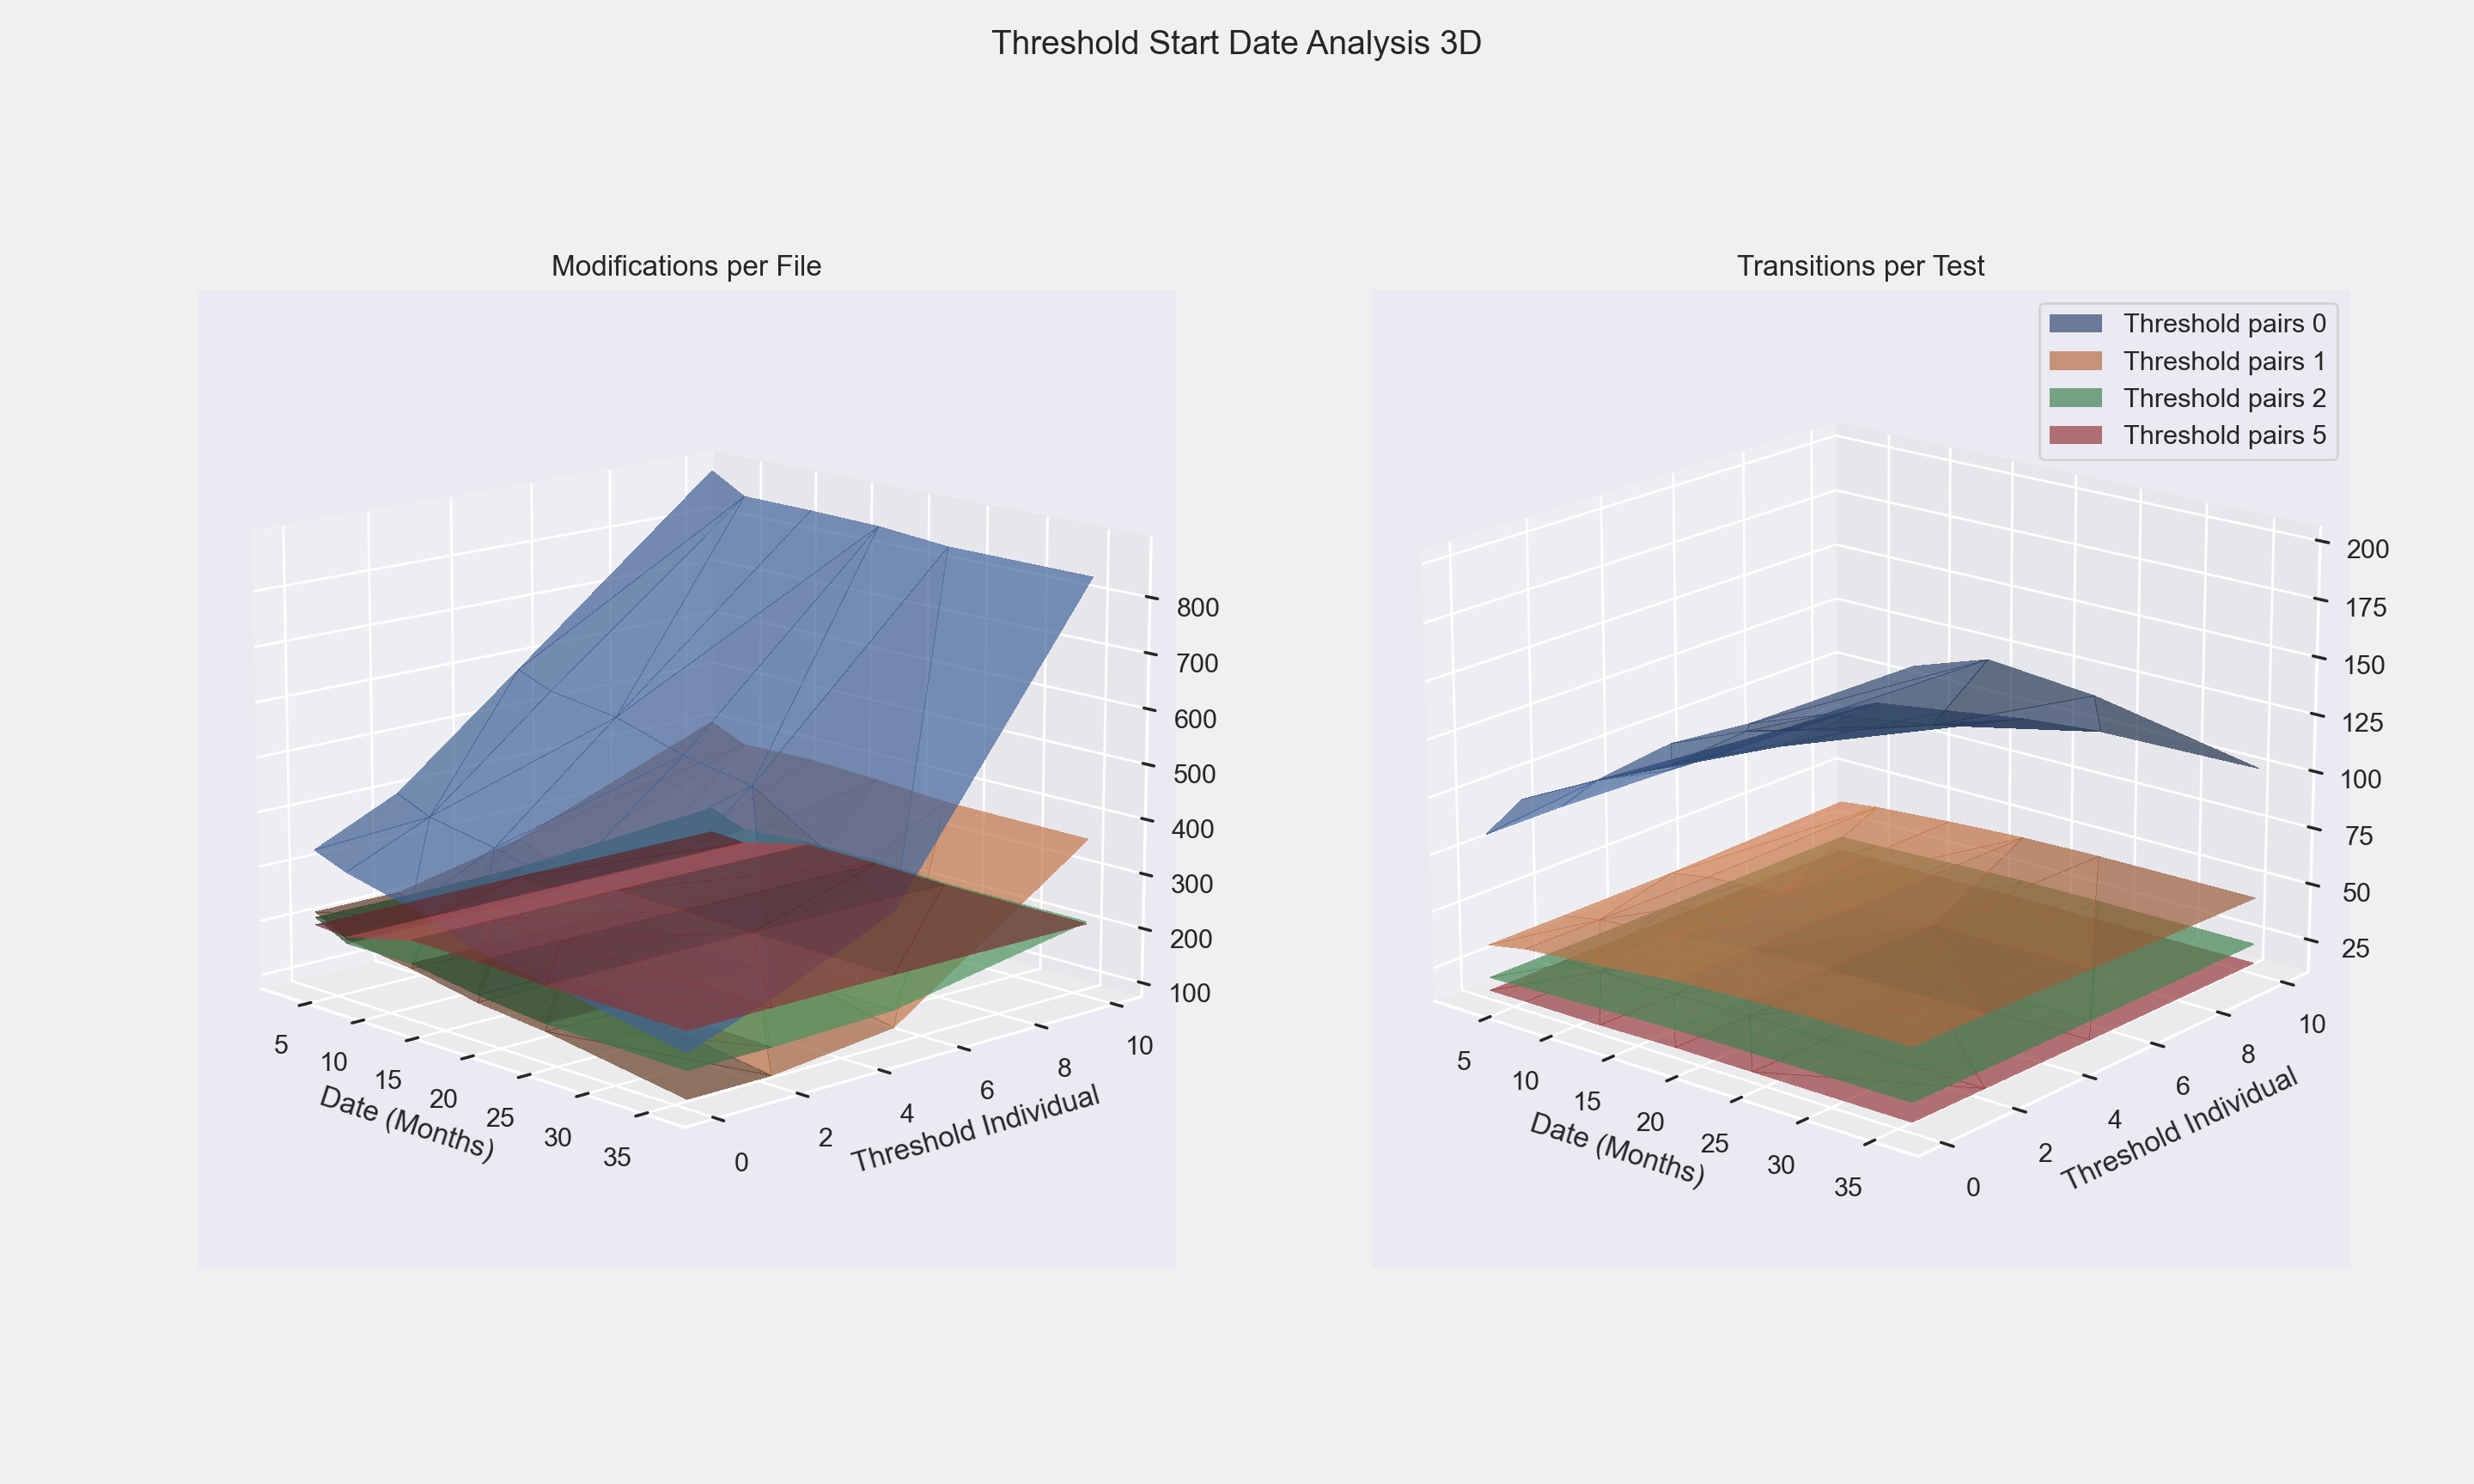
\includegraphics[width=8cm]{figures/3d_data_clean.png}
	\caption{Average number of occurrences per files/tests}
	\label{surf}
\end{figure}

In the first plot, the parameter that influences the most the average modifications per file is the individual threshold, that when is high, only the most often files prevail. However, from the initial 10800 files, only 300 remain. So there is a compromise between having an expressive dataset with only very frequent pairs and having a broader scope of valid commits. 
In both plots, for a pair threshold of 1, it is possible to see increases in the density, whilst making sure relevant files and tests are not being dropped. 

\subsection{Evaluation Metric}

the metric is the APTD

\section{Results}

\subsection{Training}

After framing the problem and having the data ready and clean, a baseline was established for training NNE-TCP for the first time. Then, the algorithm is evaluated by predicting test orderings for 100 unseen commits

\begin{figure}[h]
	\centering
	\includegraphics[width=8cm]{figures/baseline.png}
	\caption{Baseline Approach: Embedding size - 100, Negative ratio - 2, batch size - 5 commits, Task - Regression and epochs - 10}
	\label{surf}
\end{figure}

By taking the mean of the distribution the result is $ APFD = 0.66 \pm 0.19$, and for a first approach it represents a positive result, since ordering test-cases randomly, on average would yield an $APFD ~0.5$. 

\subsection{Cross-Validation}

Now that the model is trained, the next step is to account for overfitting or underfitting, or in other words, making sure the algorithm can generalize the results and not simply perform well on the training data or the model is not complex enough to adjust to the relations present in the data. 
By using Scikit Learn's KFold cross validation feature, the training set can be divided into 10 separated subets called \textit{folds}, then the model is trained 10 times, picking a different fold for evaluation every time, while the other 9 are used for training. The one fold is called the \textit{validation-set} and, if the model is not underfitting or overfitting the data, the loss and the metric on the training set should be always close to the validation set. If the curve of the validation set is above the training set's, then there is underfitting, otherwise there is overfitting. Figure \ref{cv} shows the evolution of the loss function and the metric (in this case, the Mean Absolute Error) for 10 epochs, for the baseline approach trained above.

\begin{figure}[h]
	\centering
	\includegraphics[width=8cm]{figures/cv_scores_sgd_reg.png}
	\caption{Cross Validation}
	\label{cv}
\end{figure}


Although there are discrepancies between the full line (training set) and the dashed line (validation set), it is possible to validate this model and say that there is slight overfitting. 

\subsection{Fine-Tuning}

After training our model and accounting for overfitting, it is time to find the best combination of parameters that maximize our metrics. To determine them, a search in a grid was conducted, by making combinations between the values for each parameter.
These parameters represent a gross approximation and likely do not correspond to their optimal value.  Hereafter, if not stated otherwise, the same set of parameters are used throughout the paper. 
Table \ref{paramtune} shows an overview of the chosen parameters and figure \ref{best_result} depicts the evaluation result.

\begin{table}[h]
	\begin{tabular}{cclllcllll}
		\hline
		\textbf{Parameter} & Embedding Size & Negative Ratio        & Batch Size            & Nb\_Epochs             & Task       & Optimizer               & Start Date                     & Threshold Individual  & Threshold Pairs       \\ \hline
		\textbf{Value}     & 200            & \multicolumn{1}{c}{1} & \multicolumn{1}{c}{1} & \multicolumn{1}{c}{10} & Regression & \multicolumn{1}{c}{SGD} & \multicolumn{1}{c}{1 year ago} & \multicolumn{1}{c}{5} & \multicolumn{1}{c}{1} \\ \hline
	\end{tabular}
	\caption{Optimal found Parameter Values}
	\label{paramtune}
\end{table}


\begin{figure}[h]
	\centering
	\includegraphics[width=8cm]{figures/best.png}
	\caption{Best APFD distribution - Maximum mean value }
	\label{best_result}
\end{figure}

Configuring the model with the parameters presented in Table \ref{paramtune}, the best result achieved was $APFD = 0.74 \pm 0.17$, which corresponds to an increase of $48 \%$ when compared to a random approach.  


\subsection{Entity Representation}

\begin{figure}[t]
\centering
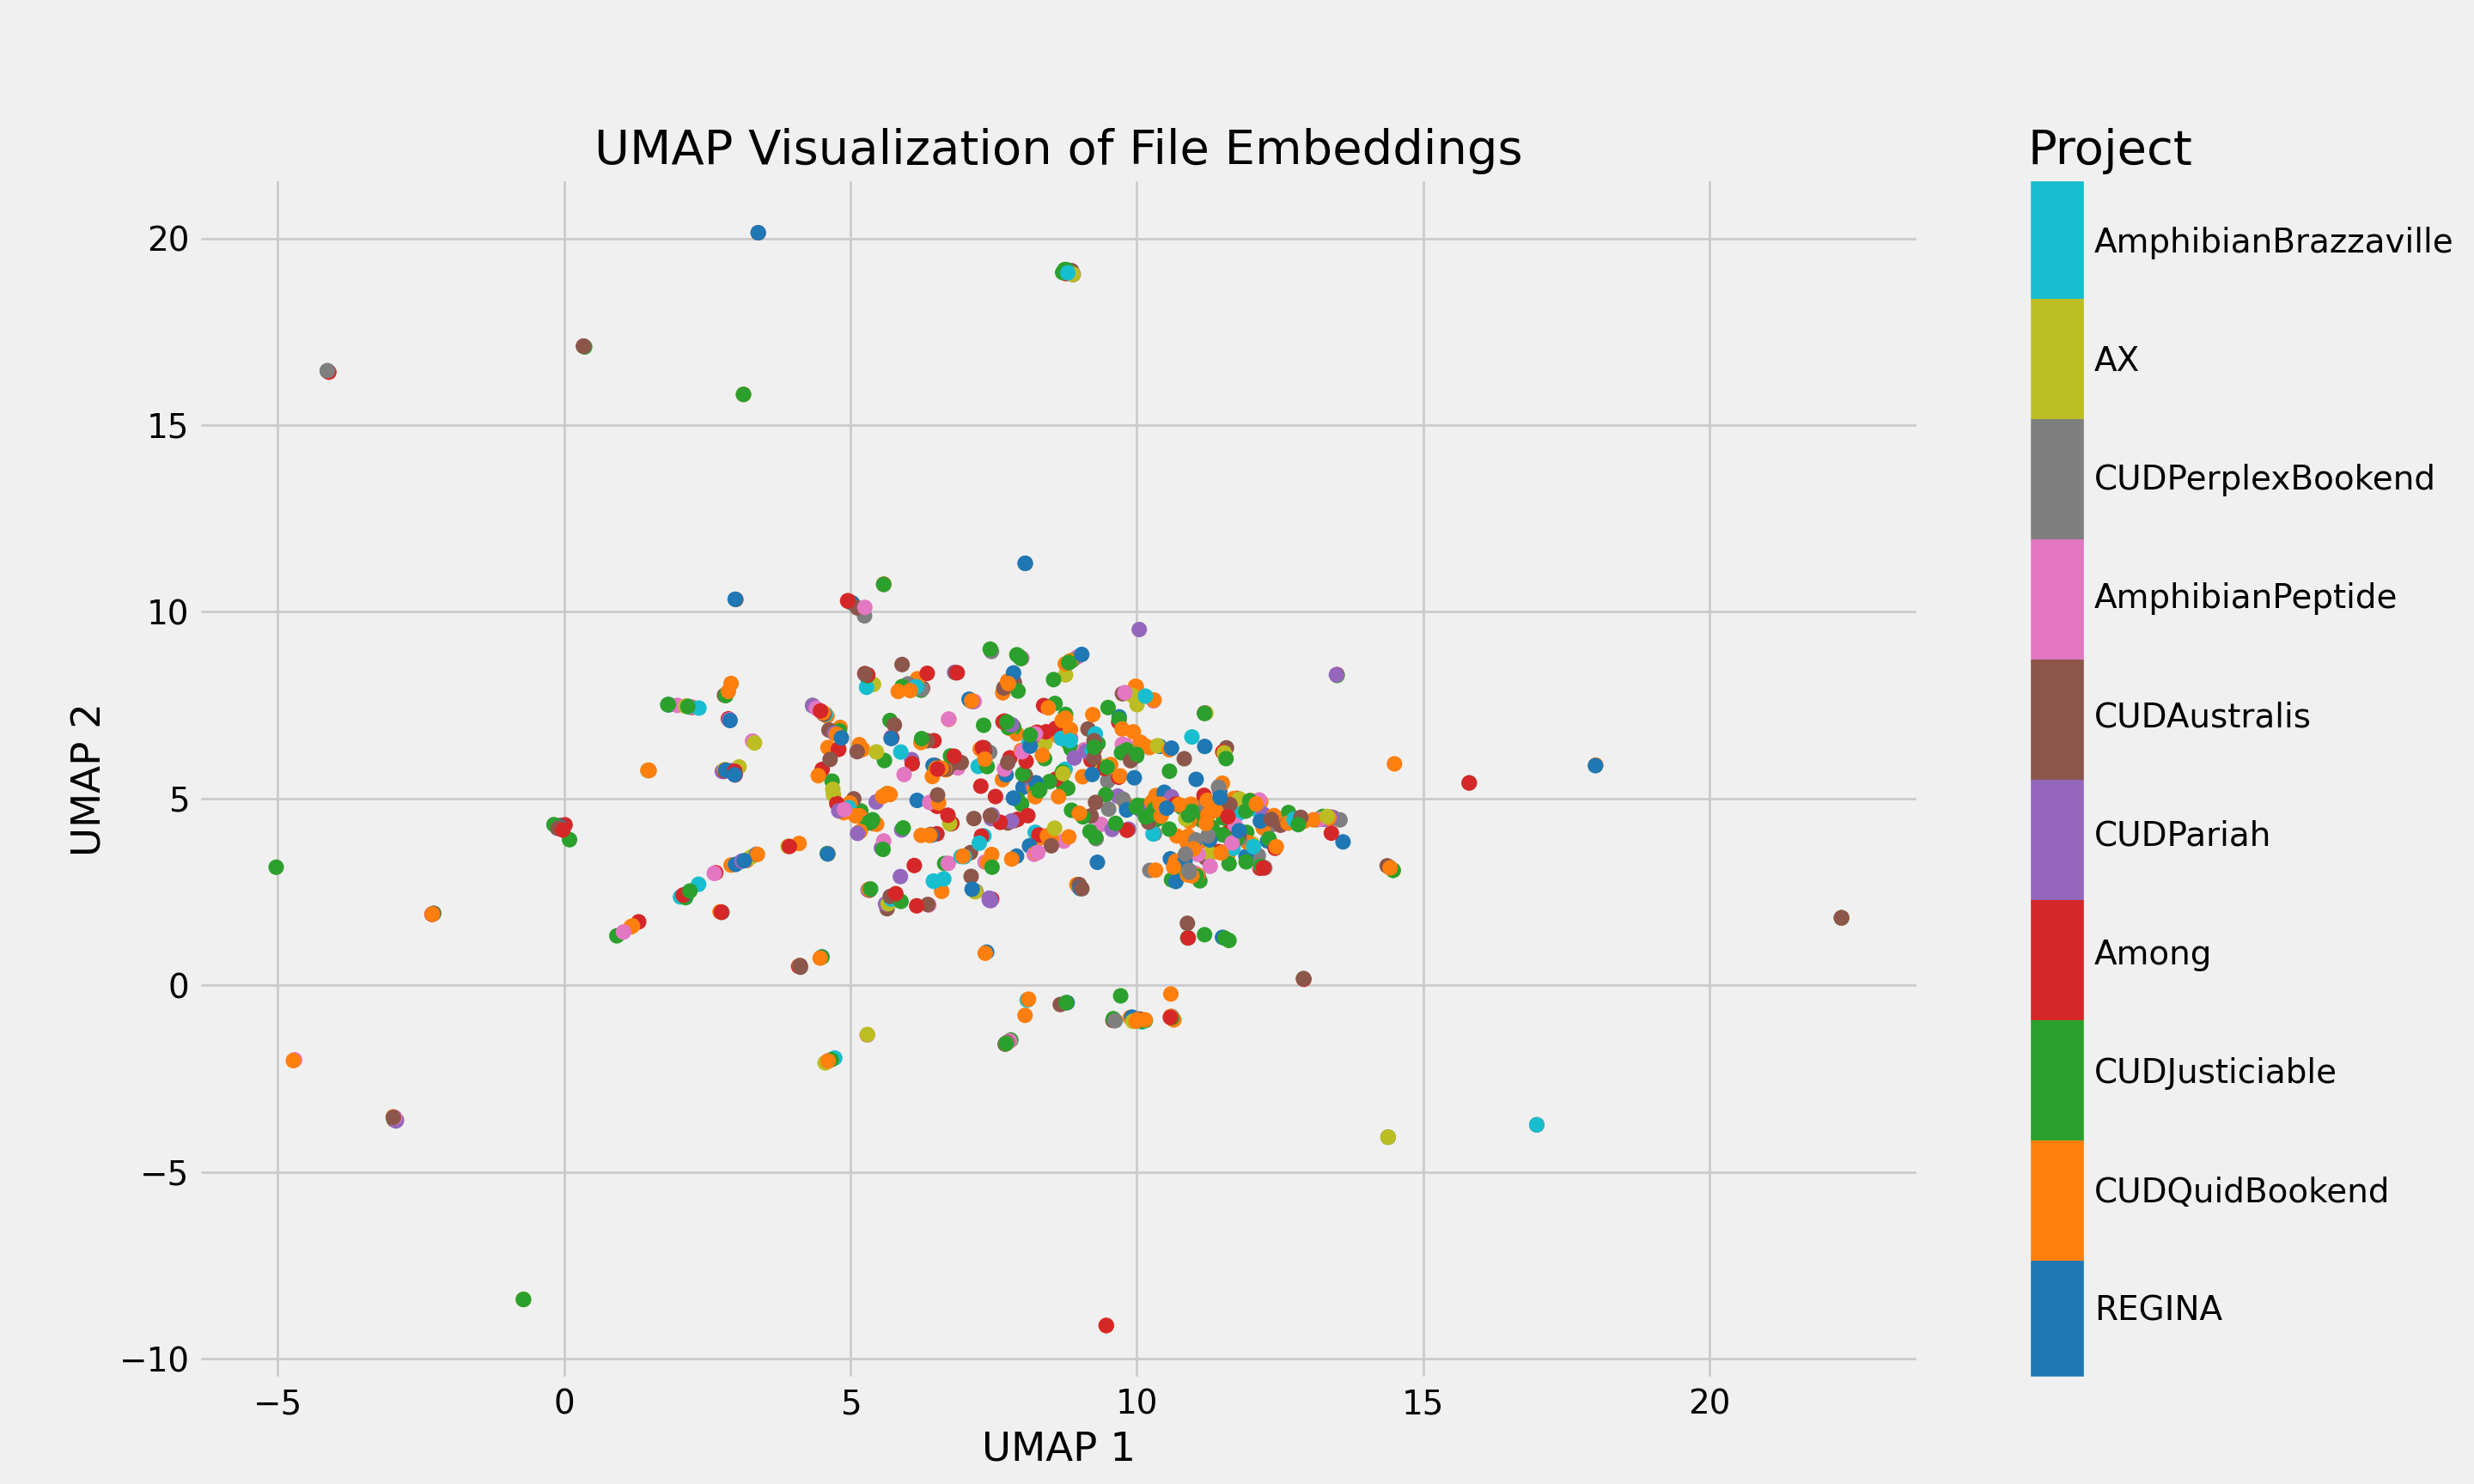
\includegraphics[width=\linewidth]{figures/best_emb_UMAP_files.png}
\label{fig:sub1}
\end{figure}

\begin{figure}[t]
	\centering
	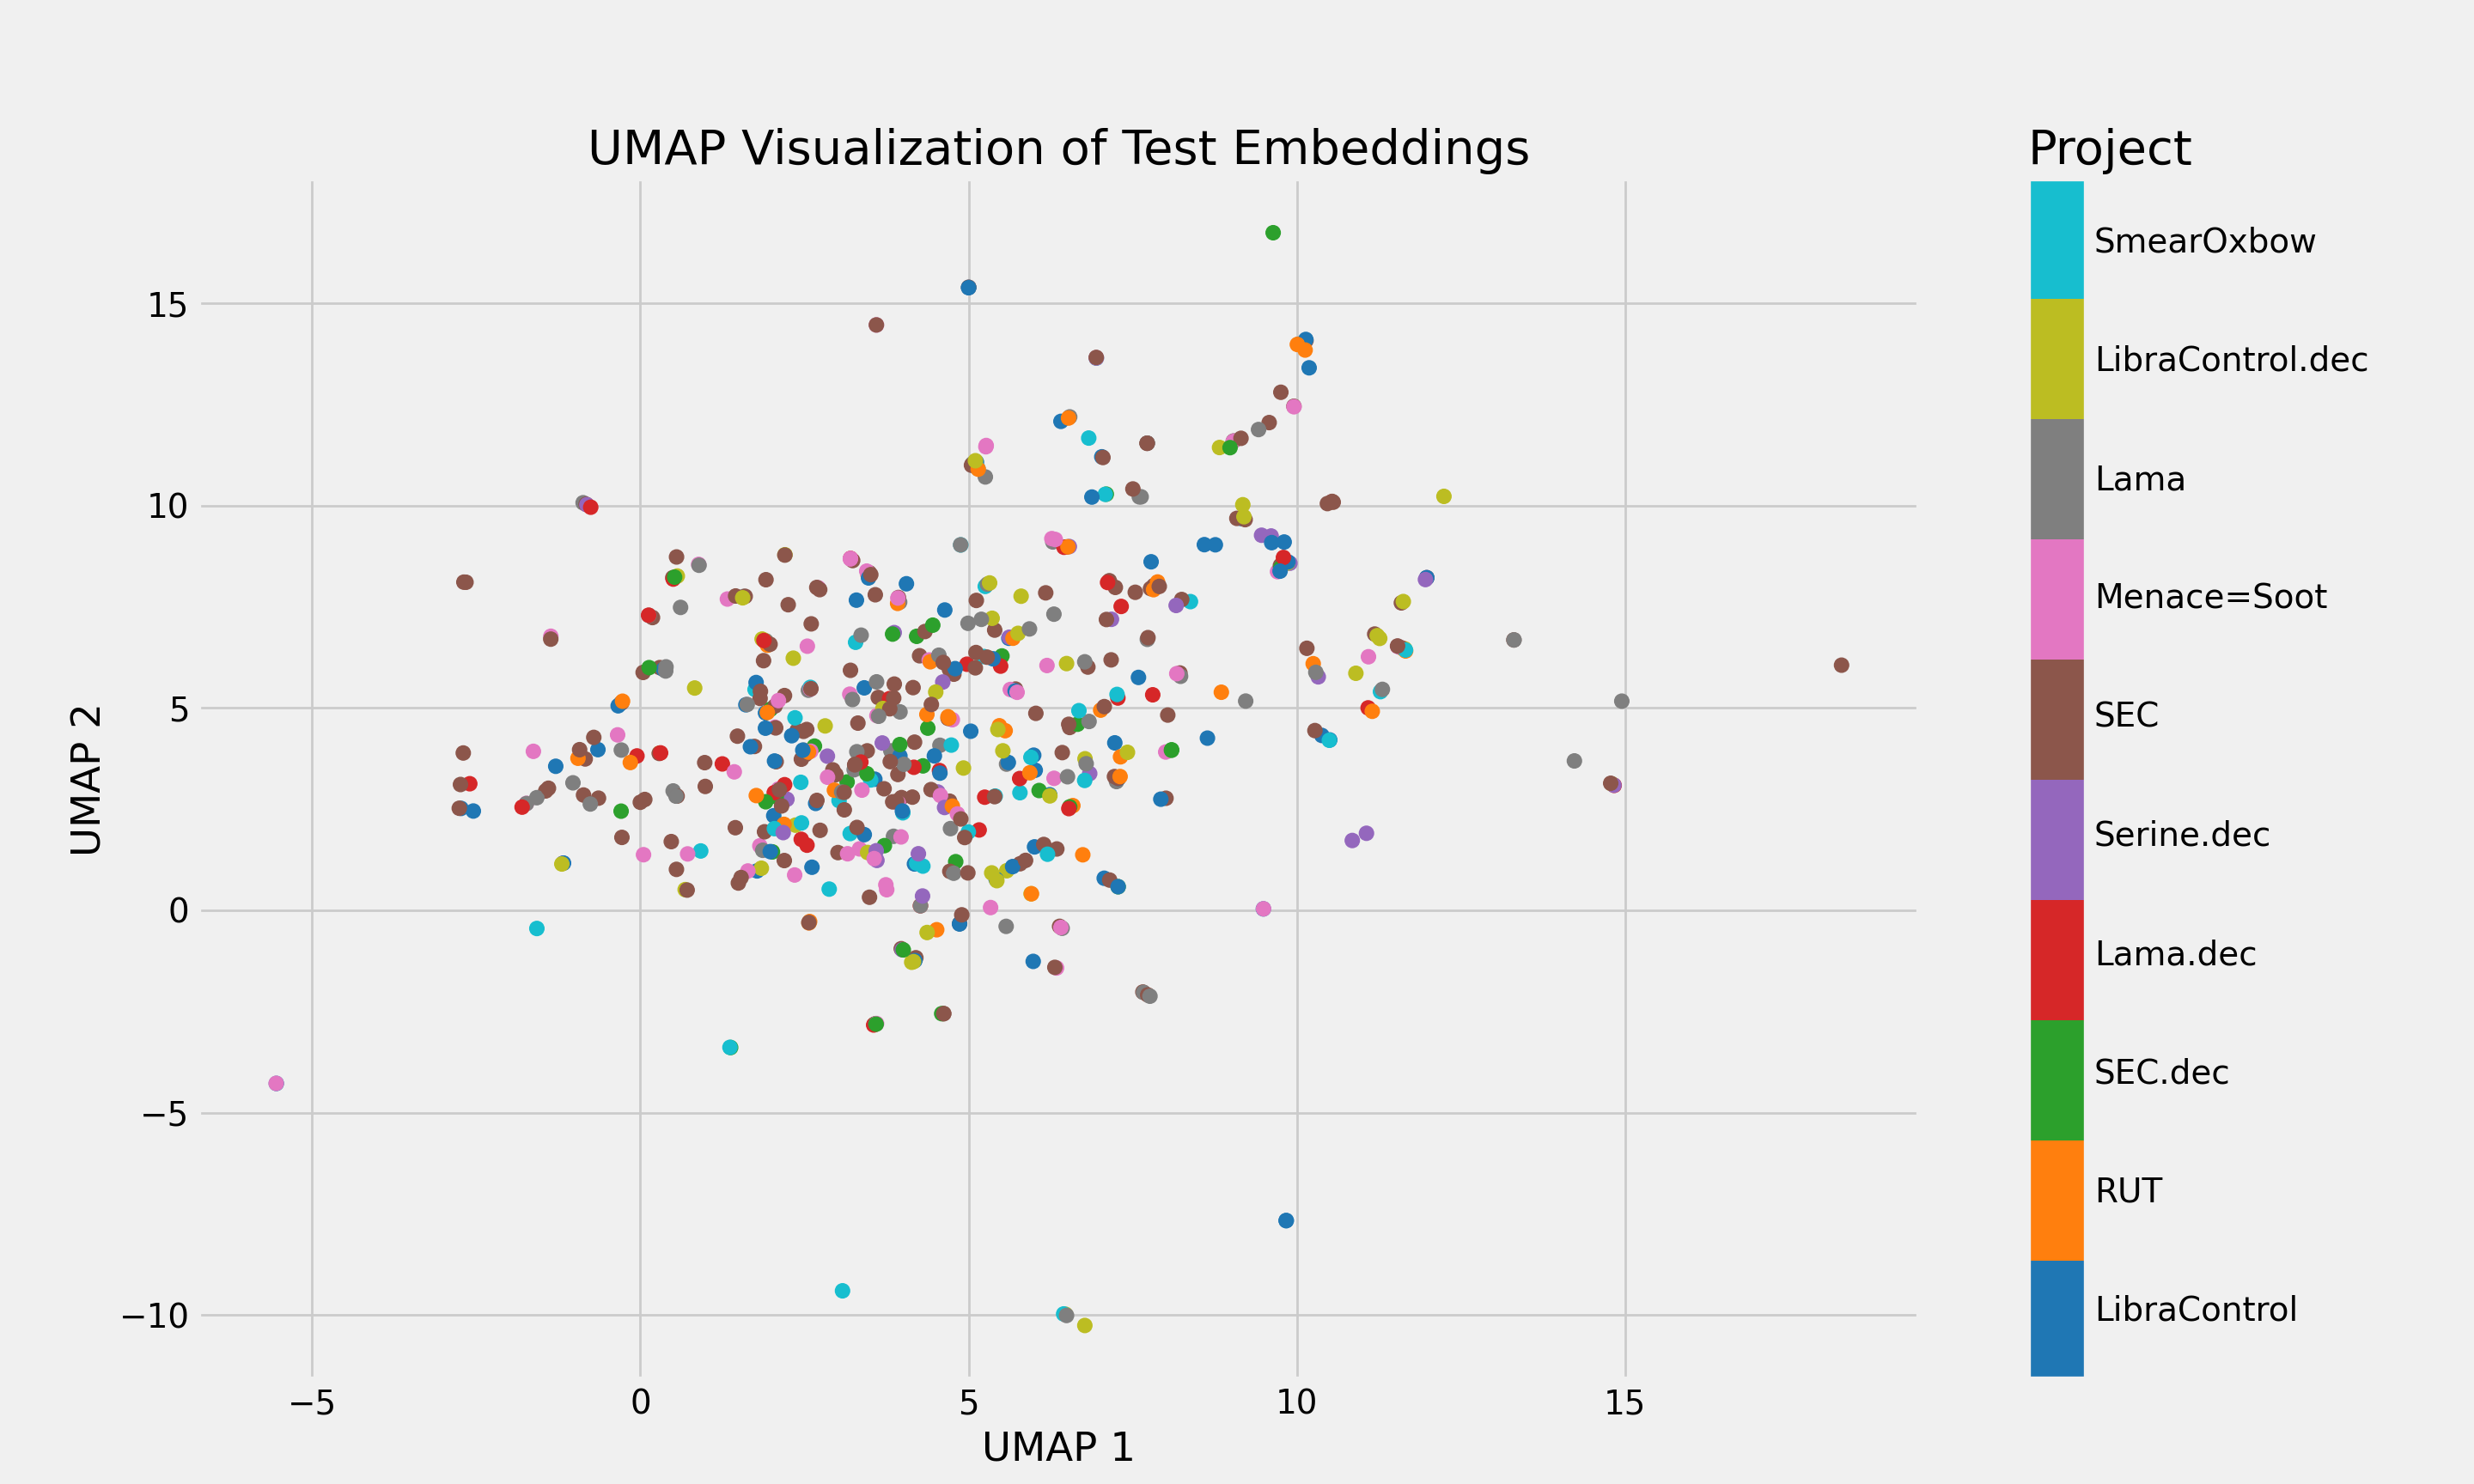
\includegraphics[width=\linewidth]{figures/best_emb_UMAP_test.png}
	\label{fig:sub2}
\end{figure}



The advantage of using Embedding Models is that beyond solving a Supervised Learning Problem, the results can be visualized in 2D space. Figure \ref{fig:sub1} shows the embedding representation for files and test-cases, by using the manifold reducing technique UMAP and by labelling files and tests appropriately. Due to limitations in the data, the available labels that can be extracted are the directory where each file/test is stored and only for tests an identifier written in the name of the tests pointing to functionality \footnote{information provided by domain expert}. Figure \ref{fig:sub2} shows labelled embeddings representation, for the ten most frequent labels. Also, labels were made by humans, hence some of them are not written in non-uniform  format and are incorrect or uninformative.
\\

One general observation is that embedding representation and the current labelling show no correlation. Entities are grouped by likelihood of being involved in transitions together and in the case of modified files, that does not occur for the ones that are kept in the same directories. 

\subsection{Threats to Validity}
\textbf{Internal.} The first threat to validity is associated with randomness when training the model, which was mitigated by using cross-validation, that performs training multiple times. 
Another threat can derive from errors associated with our code implementation. Both Scikit-learn and Keras are well established frameworks used for Machine Learning and furthermore, the code is open-source and available online \footnote{https://github.com/jlousada315/NNE-TCP} for reproduction and inspection purposes. \\

\textbf{External.} The evaluation made is based on a single development environment, which is a major limitation considering the amount of real-world scenarios where CI is applied. This threat has to be addressed by running more experiments on data from several industries, with different development paces, team size, resources, etc. To contribute to more data availability, publication of the dataset used in this paper is being authorized. \\

\textbf{Construct.} In real-world complex CI systems, sometimes test-cases change status due to extraneous reasons: system dependencies of several platforms can affet the outcome of a test , the infrastructure where tests are run can suffer critical failures or malfunctions, some tests can fail to produce the same result each time they are run (flaky tests). Therefore it is not certain that a test case changed status, because a certain file was modified. \\
Regarding the features used for training, our model only looks at the link between modified files and tests, whereas in real life additional features may have a positive impact on the capability to make better predictions, e.g. commit author, execution history of each test - test that are not applied in a long time have more chance of changing status and tests that have failed recently are more likely to fail again -, test age, etc. 
To better validate the results achieved by NNE-TCP it should be compared with other Machine Learning based Test Case Prioritization techniques described in the literature.


